
\clearpage
\section{Расчет досягаемости геометрии}\label{main_part}
Основным приемом отсечения геометрии является отсечение ее по коэффициенту самозатенения, который вычисляется по следующему алгоритму.

Первым шагом алгоритма будет упрощение данных о геометрии. Упрощение сводит каждый полигон к окружности, имеющей координаты центра, нормаль и площадь, оно позволит сильно упростить расчеты того, насколько одна из поверхностей затеняет другую. Центром окружности является усредненное значение координат всех точек полигона.
\begin{equation}
	\sum_{i=0}^{n} x_i / n
\end{equation}

Нормаль вычисляется по трем любым точкам ($a$, $b$, $c$) по следующей формуле:
\begin{equation}\begin{split}
	w = {(c-a) \times (b-a)} \\
	n = w \cdot 1 / \sqrt{\sum_{i=0}^{n} {w_i^2}}
\end{split}\end{equation}

Площадь треугольника вычислим по формуле Герона.
\begin{equation}\begin{split}
	p= {{a+b+c}\over{2}} \\
	S=\sqrt{p(p-a)(p-b)(p-c)}
\end{split}\end{equation}

\begin{figure}[h]
	\center
	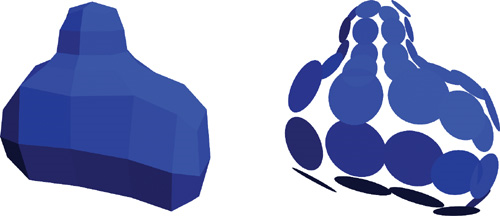
\includegraphics[width=0.5\textwidth]{14_ambient_occlusion_02}
	\caption{Перевод полигонов в диски той же площади}\label{fig:ao02}
\end{figure}
Ambient occlusion -- полезная техника для затенения объектов, которая используется в современной графике. Благодаря ambient occlusion получаются мягкие тени за счет затемнения поверхностей, которые частично видны с некоторой внешней точки. Эта техника также включает в себя расчет коэффициента досягаемости полигона к окружению, или, другими словами, число обратное числу пересечений его с другими полигонами в полусфере перед первым.

Будем называть элемент, на который падает тень ресивером, а элемент бросающий тень  -- эммитером. Для расчетов количества тени, которая бросается эммитером на ресивер используется формула, основанная на телесном угле для ориентированного диска 


\begin{equation}
	{{r\cos{\Theta_E \max(1, 4\cos{\Theta_R})}}\over{\sqrt{{A\over\pi} + r^2}}}
	\label{em_rec}
\end{equation}
Где $А$ -- площадь эммитера\\
$E$ -- эммитер\\
$R$ -- ресивер\\
$RE$ -- отрезок, соединяющий центры дисков\\
$r$ -- длина отрезка RE, расстояние между дисками\\
$\Theta_R$ -- угол между нормалью ресивера и отрезком ER\\
$\Theta_E$ -- угол между нормалью эммитера и отрезком ER\\

\begin{figure}[h]
	\center
	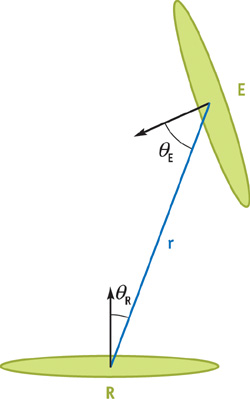
\includegraphics[width=0.3\textwidth]{14_ambient_occlusion_03}
	\caption{визуализация расположения эммитера и ресивера и эелементов уравнения \ref{em_rec}}\label{fig:ao03}
\end{figure}

Если вычислить значение затенения каждого полигона с каждым другим, то суммарная величина и будет являться коэффициентом самозатенения этого полигона. Полигоны, имеющие относительно низкие значения этого коэффициента более вероятно являются оболочкой, нежели находятся внутри и наоборот. Для полигонов, находящихся внутри модели коэффициент будет близок в единице. Полигоны, имеющие некоторые средние значения коэффициента могут как находится внутри модели, так и являться оболочкой. Для корректного удаления такой геометрии при отсечении используется вводимая пользователем граница отсечения. В случае слишком агрессивного, или наоборот, отсечения можно отменить сделанные изменения и повторить процедуру с другим коэффициентом. Пересчета самозатенения для этого не требуется, поэтому процедура выполняется в реальном времени.

\clearpage
\section{General-purpose graphics processing units}
Большинство задач, связанных с графикой и триангулированной геометрией требуют вычислений с большим количеством операций. Современные графические адаптеры устроены таким образом, чтобы выполнять огромное число достаточно простых, не связанных друг с другом, операций одновременно.

Расчеты, в создаваемом, в рамках настоящей работы, приложении, было решено выполнять с помошью GPU.

Существует большое количество технологий для выполнения таких расчетов, рассмотрим некоторые из них.

\subsection{Compute shader}
Шейдер -- программа написанная на особом языке, предназначенная для выполнения процессором видеокарты. Шейдеры бывают нескольких видов:
\begin{itemize}
\item Fragment shader
\item Vertex shader
\item Compute shader
\item Tesselation control shade
\item Tesselation evaluation shader
\end{itemize}

Использование геометрических, а в некоторых случаях и фрагментных, шейдеров открыло возможность для расчетов общего назначения с появлением программируемого графического конвеера, взамен статическому. Сами фрагментные шейдеры используются для вычисления цветов пикселей, применения затенения и текстурирования к ним, во время растеризации полигонов видеокартой. В современных GPU может находиться до нескольких тысяч ядер процессора, способных выполнять такие шейдеры. Задача, решаемая в рамках ВКР хорошо распараллеливается, что позволяет получить все преимущества от параллельных вычислений на GPU. Недостатком использования вычислительных шейдеров являются сложности с использованием памяти. Фактически единственным способом как передачи больших массивов данных в программу, так и получения результатов ее работы, является передача их через текстуру, что не всегда является удобным.

\subsection{OpenCL}
OpenCL -- это фреймворк для написания компьютерных программ, основанных на параллельных вычислениях. OpenCL задумывался для работы в гетерогенной вычислительной среде и абстрагирует платформу, на которой производятся вычисления (GPU, CPU) и производителя устройства, предоставляя единый интерфейс.

OpenCL первоначально был разработан в компании Apple Inc. Apple внесла предложения по разработке спецификации в комитет Khronos. 16 июня 2008 года была сформирована рабочая группа Khronos Compute для разработки спецификаций OpenCL. 9 декабря 2008 года организация Khronos Group представила первую версию стандарта.

OpenCL предоставляет гораздо более удобный интерфейс для работы с массивами входных и выходных данных, было принято решение использовать его в качестве основного инструмента вычислений.

\clearpage
\section{Реализация расчета самозатенения}\label{main_part}
\subsection{Первичная реализация}
Первичная реализация была выполнена с помошью встроеных средств языка программирования C\#. Число потоков выполнения определяется числом ядер центрального процессора, затем обрабатываемая модель разделяется на соответствующее число частей и вызываются потоки расчетов, кажому из который достается свой фрагмент модели. Листинг программы расчетов представлен в приложении В. Средняя скорость расчета для модели в 200000 полигонов составила 00:01:40.2732. Учитывая то, что модели аттракторов, печатаемые на кафедре на 3D принтеры имеют до нескольких миллионо полигонов было принято решение оптимизировать скорость вычислений с помошью более продвинутых вычислительных технологий. 
\subsection{Реализация с помощью compute shader}
Следующей реализацией алгоритма была реализация на языке GLSL. Производительность была заметно увеличена за счет числа одновременно выполняемых расчетов и составила всреднем 00:00:30.0788. Производительность была увеличена примерно в 3 раза, однако это все еще было решено недостаточным. Так же очевидными недостатками подхода можно выделить ограничения на обрабатываемые модели, которое обусловлено ограничением видеокарты на одновременно обрабатываемую геометрию (у современных видеокарт порядка 2 миллионов вершин) и зависание работы GUI и OC в следствие высокой нагрузки на GPU, что переодически приводило ОС к решению о зависании видеодрайвера и его перезагрузке, что прерывало расчеты. Разделение расчетов на небольшие части полностью убирало выигрыш по производительности от использования вычислительных шейдеров.
\subsection{OpenCL реализация}
Финальной реализацией стала реализация с помошью фреймворка OpenCL. Среднее время выполнения расчетов для модели, состоящей из 200000 полигонов, всреднем, составило 00:00:02.5196, что составило прирост в 40 раз по сравнению с изначальной реализацией.  Листинг программы на диалекте языка C99 представлен в приложении Б. Вычисления состоят из двух этапов:
\begin{itemize}
\item Предрасчет площадей полигонов (floatSquareDivPi)
\item Расчет самозатенения (floatAO)
\end{itemize}

Предрасчет площадей, непосредственно перед расчетом самозатенения, позволяет значительно увеличить производительность за счет использования дополнительной памяти, но благодаря этому расчет площади производится только число раз, равное числу полигонов, а не квадрату этого числа, как в случае расчета непосредственно во время расчета самозатенения. Примери работы приложения и интерфейс предсавлен в приложениях.

\clearpage
\section{Пример работы и интерфейс приложения}
\begin{figure}[h]
	\center
	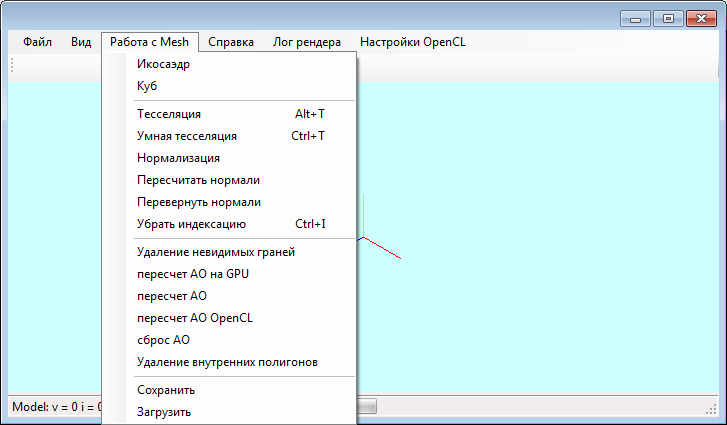
\includegraphics[width=1\textwidth]{int}
	\caption{интерфейс приложения}\label{interface}
\end{figure}
На рисунке \ref{interface} представлен интерфейс приложения. Основной частью которого является интерактивный экран, голубого цвета, на котором отображается модель, обработка которой осуществляется в текущий момент. Рендер модели может производиться в режиме заливки и wireframe. Возможно выбрать способ заливки -- затенение и самозатенение. В режим затенением является комбинацией нормального затенения и самозатенения. Режим самозатенения используется для удобного выбора коэффициента отсечения геометрии т.к. позволяет визуально определить что отсекается.

Так же в интерфейсе присутствует меню, состоящее из нескольких пунктов:
\begin{itemize}
\item Файл. Позволяет вызвать диалоги сохранения и загрузки файлов.
\item Вид. Выбор настроек одображения модели.
\item Работа с Mesh. Основные возможности программы. Позволяет тесселировать геометрию несколькими способами для более точного отсечения, убрать индексацию для индексированных моделей, а так же расчитать коэффициент самозатенения и вызвать диалог отсечения геометрии.
\item Справка. Описание работы программы.
\item Лог рендера. Выводит информацию о ошибках шейдеров, которые используюстя для вывода модели, а так же вычислительных шейдеров и ошибки OpenCL
\item Настройки OpenCL. Позволяет выбрать платформу, на которой будет производиться вычисления фреймворком OpenCL.
\end{itemize}

В нижней строке состояния отображается информация о модели, такая как число вершин и индексов модели, а так же строка прогресса расчета самозатения.

\begin{figure}
	\center
	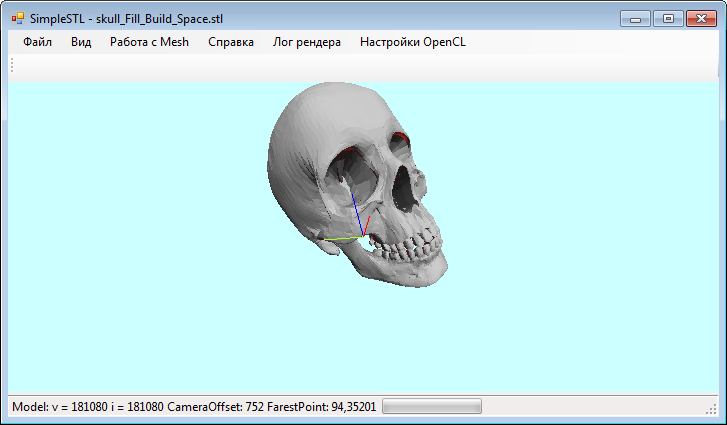
\includegraphics[width=1\textwidth]{scull2}
	\caption{Модель до расчета самозатенения}\label{scull2}
\end{figure}
\begin{figure}
	\center
	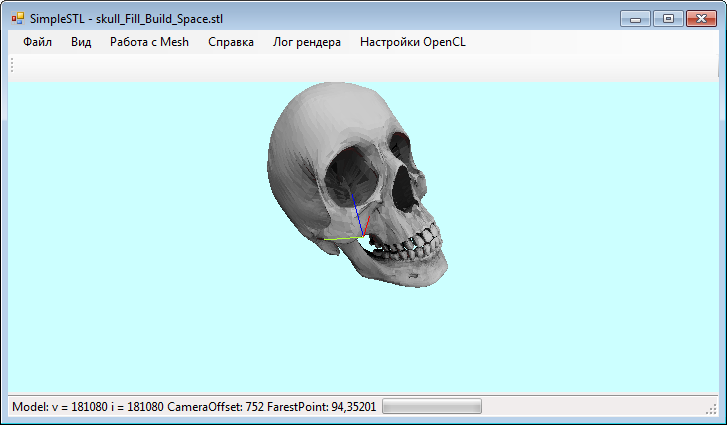
\includegraphics[width=1\textwidth]{scull1}
	\caption{Модель с расчитанным самозатенением}\label{scull1}
\end{figure}
\begin{figure}
	\center
	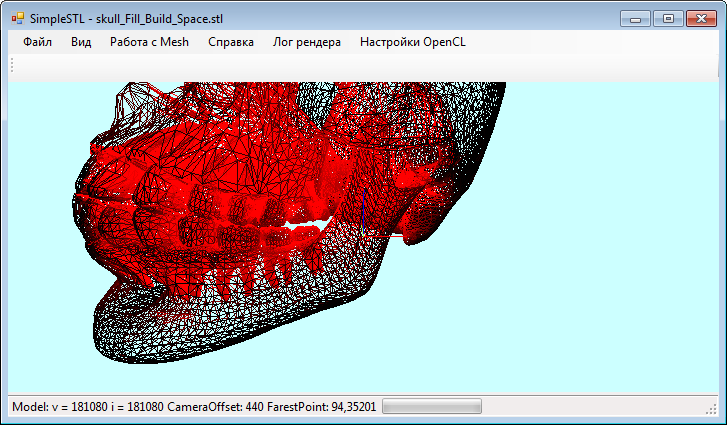
\includegraphics[width=1\textwidth]{scull3}
	\caption{Самозатенения для геометрии, находящейся внутри модели}\label{scull3}
\end{figure}
\begin{figure}
	\center
	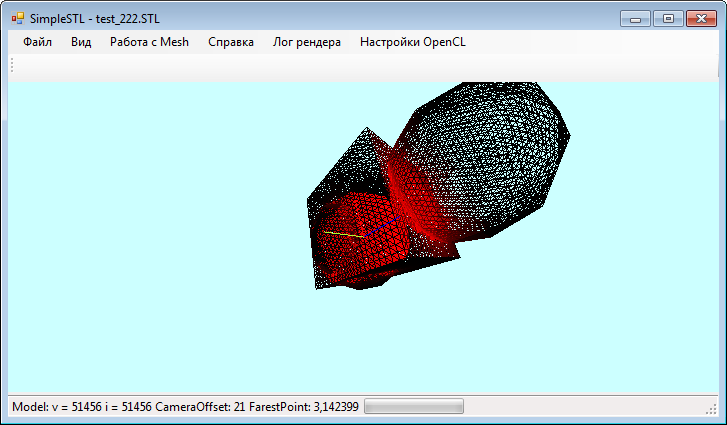
\includegraphics[width=1\textwidth]{atr2}
	\caption{Модель сфер, пересекающихся с кубом до отсечения геометрии}\label{atr2}
\end{figure}
\begin{figure}
	\center
	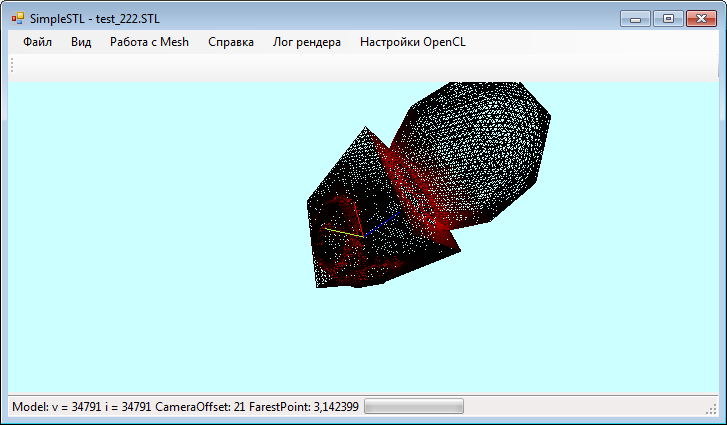
\includegraphics[width=1\textwidth]{atr3}
	\caption{Модель сфер, пересекающихся с кубом после отсечения геометрии}\label{atr3}
\end{figure}